\documentclass{article}
\usepackage[utf8]{inputenc}
\usepackage{multicol}
\usepackage{amsmath}
\usepackage{float}
\usepackage{epsfig,graphicx}
\usepackage{xcolor,import}
\usepackage{subcaption}
\usepackage[font=small,labelfont=bf]{caption}
\usepackage{siunitx}
\usepackage[german]{babel}
\usepackage{textcomp}
\usepackage{mathtools}

\begin{document}


\thispagestyle{empty}
			\begin{center}
			\Large{Fakultät für Physik}\\
			\end{center}
\begin{verbatim}


\end{verbatim}
							%Eintrag des Wintersemesters
			\begin{center}
			\textbf{\LARGE SOMMERSEMESTER 2015}
			\end{center}
\begin{verbatim}


\end{verbatim}
			\begin{center}
			\textbf{\LARGE{Physikalisches Praktikum II}}
			\end{center}
\begin{verbatim}




\end{verbatim}

			\begin{center}
			\textbf{\LARGE{PROTOKOLL}}
			\end{center}
			
\begin{verbatim}





\end{verbatim}

			\begin{flushleft}
			\textbf{\Large{Experiment 3: Radioaktivität}}\\
							%Experiment Nr. und Titel statt den Punkten eintragen
			\LARGE{}	
			\end{flushleft}

\begin{verbatim}

\end{verbatim}	
							%Eintragen des Abgabedatums, oder des Erstelldatums des Protokolls
			\begin{flushleft}
			\textbf{\Large{Datum:}} \Large{27.03.2015}
			\end{flushleft}
			
\begin{verbatim}
\end{verbatim}
							%Namen der Protokollschreiber
		\begin{flushleft}
			\textbf{\Large{Bachleitner Veronika, Grafendorfer Erik}} 
			\end{flushleft}

\begin{verbatim}


\end{verbatim}
							%Kurstag und Gruppennummer, zb. Fr/5
			\begin{flushleft}
			\textbf{\Large{Kurstag/Gruppe:}} \Large{FR/1}
			\end{flushleft}

\begin{verbatim}






\end{verbatim}
							%Name des Betreuers, das Praktikum betreute.
			\begin{flushleft}
			\LARGE{\textbf{Betreuer: \Large{HUMMER}}}		
			\end{flushleft}
			
\section{Aufgabenstellung}

\section{Theorie}
\subsection{}

\section{Aufbau}

\section{Durchführung}

\section{Ergebnisse}


\subsection{Körpereigene Radioaktivität}
Wir haben $140g$ Kalium im Körper (ausgehend von $70kg$ Körpergewicht).
Davon sind
$$
140g\cdot 0.000117=1.638\cdot10^{-2}g \\
$$
Kalium 40.\\
Kalium40 hat $40\frac{g}{mol}$. Also haben wir \\
$$4.095\cdot10^{-4}mol$$ Kalium 40 im Körper.\\
\\
Wenn wir dies mit der Avogadro-Konstante multiplizieren erhalten wir:\\
$$2.46607\cdot 10^{20}$$ Atome Kalium 40.\\
\\
Mit einer Halbwertszeit von $T_{\frac{1}{2}}= 1.28 \cdot 10^{9}a=4.039\cdot 10^{16}s$ \\
bekommen wir die Lebensdauer $$\tau=\frac{T_{1}{2}}{\log{2}}=\lambda^{-1} \Rightarrow \lambda=1.7159 \cdot 10^{-17}$$
\\
Daraus gelangen wir schließlich zu dem Ergebnis, dass die körpereigene Aktivität folgenden Wert hat:
$$A=N\cdot \lambda = 4.2317\cdot 10^{3} \textrm{ Ereignisse / Sekunde}$$
\subsection{Szintillationszähler}
Bei der Messung von Natrium 22 sehen wir Peaks bei $(513.10 \pm 5.00)\si{keV}$ und $(1275.97 \pm 27.80)\si{keV}$. Die Skala wird auf diese Energien kalibriert.\\
\\
Nachdem eine unbekannte Probe in den Behälter gegeben wurde messen wir wieder und sehen nun Peaks bei $(1181.16 \pm 7.90)\si{keV}$ und $(1333.78 \pm 14.29)\si{keV}$.\\
Aufgrund der gemessenen Peaks stellen wir fest, dass es sich bei der unbekannten Probe um \textbf{Cobalt 60} handeln muss.

\begin{center}
\begin{figure}[H]
\begin{subfigure}{0.52\textwidth}
\includegraphics[width=0.9\linewidth]{bachgrafbild.jpg}
\caption{}
\end{subfigure}
\begin{subfigure}{0.52\textwidth}
\includegraphics[width=0.9\linewidth]{bachgrafunbekannt-peaks.eps}
\caption{}
\end{subfigure}
\caption{Die rote Linie in (a) sowie (b) ist das Gammaspektrum von Natrium 22. Die violette Linie in (b) repräsentiert Cobalt 60. Die horizontale Achse zeigt die Energie, die vertikale Achse die Zählrate.}
\end{figure}
\label{fig:szint}
\end{center}
% -- \ref{fig:name}

In Abbildung \ref{fig:szint} sieht man bei Natrium 22 (a) zwei schöne Photopeaks bei den erwarteten Energien von $(513.10 \pm 5.00)\si{keV}$ ($511\si{keV}$) und $(1275.97 \pm 27.80)\si{keV}$ ($1275\si{keV}$). Auch das Comptongebirge ist gut zu sehen; die Comptonkante befindet sich kurz vor dem zweiten Photopeak. Es gibt auch einen etwas kleineren Peak, der die Röntgenlinie darstellt, sowie einen Rückstreupeak ganz am Anfang des Spektrums.\\
In (b) bei Cobalt 60 ist ganz Ähnliches zu sehen. Es handelt sich hier wieder um zwei Photopeaks bei den erwarteten Energien von $(1181.16 \pm 7.90)\si{keV}$ ($1173\si{keV}$) und $(1333.78 \pm 14.29)\si{keV}$ ($1333\si{keV}$).

\subsection{Abstandsabhängigkeit}
%N4:131.44mm : 187 :
%N5:127.30mm : 178 :
%N6:123.22 : 199 :
%N7:115.00 : 209 :
%N8:98.50 :260 :
%N9:65.7 : 479 Ereignisse:
Die Zählrate $Z$ wurde mit dem Szintillationszähler in Abhängigkeit des Abstands von der Strahlungsquelle gemessen.\\
Den Abstand $x$ messen wir mit einer Messlehre; der reale Abstand von der Probe ist $d=x-1$.\\
\\
Da wir die Unsicherheiten der Zählraten nicht mitgeschrieben haben, vergleichen wir mit den Ergebnissen von anderen Mitstudenten. Wir sehen dort relative Unsicherheiten von bis zu $8\%$ und verwenden diese.
\\
\begin{tabular}{|r|r|l|}
\hline
$x$ ($\si{mm}, \pm 0.01$) & $d$ ($\si{mm}, \pm 0.01$) & $Z$ ($1/s, \pm 8\% $)\\
\hline
$127.30$ & $126.30$ & $178$\\
$123.22$ & $122.22$ & $199$\\
$115.00$ & $114.00$ & $209$\\
$98.50$ & $97.50$ & $260$\\
$65.72$ & $64.72$ & $479$\\
\hline
\end{tabular}

\begin{center}
\begin{figure}[H]
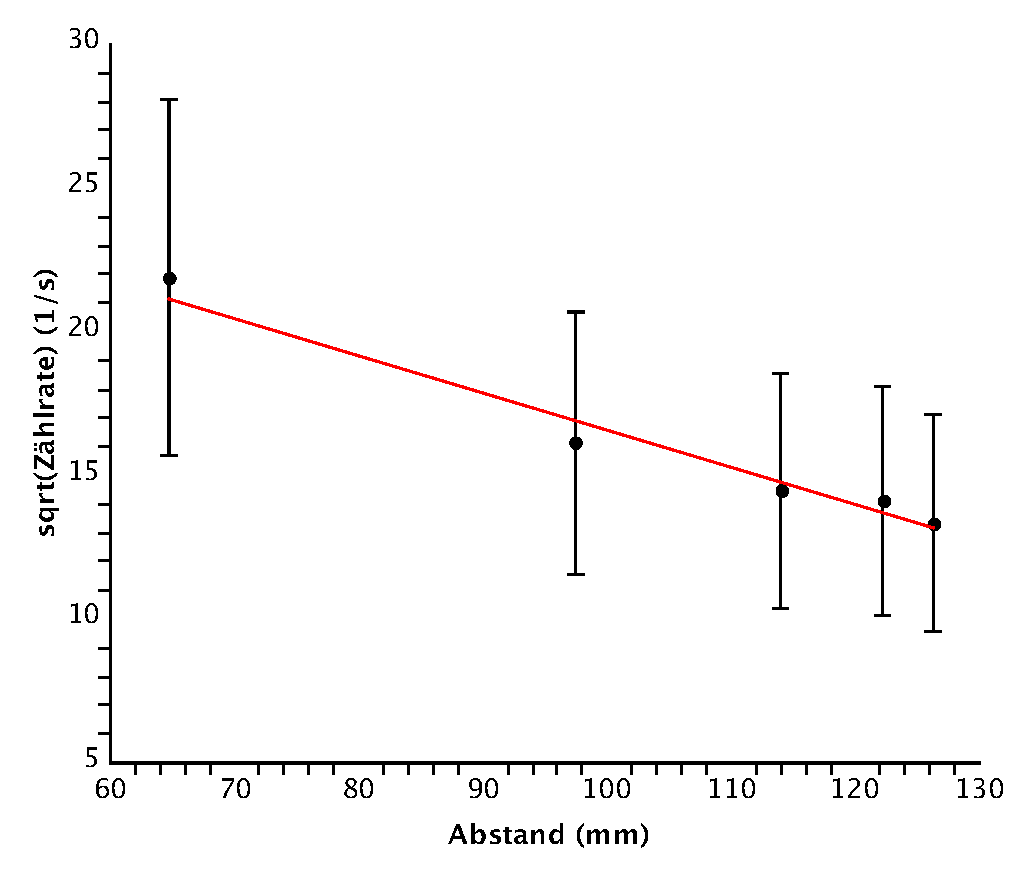
\includegraphics[scale=0.6]{abstandwurzel.eps}
\caption{Linearer Fit zur Abstandsabhängigkeit. Es wurde die Wurzel der Peak-Maxima genommen, um den linearen Fit machen zu können.}
\end{figure}
\end{center}

\subsection{Nebelkammer}
\subsection{Geiger-Müller-Zählrohr}

\section{Diskussion}																								
\end{document}
